\section*{Výsledky měření}
Měření proběhlo při pokojové teplotě ($\approx \SI{22}{\degreeCelsius}$).
Všechny uvedené odchylky jsou standardní.

\subsection*{Tlumené kmity}

Změřili jsme dobu kmitu $T$ při $R=\SI{20}{\ohm}$ v závislosti na $C$.
Výsledky jsou uvedeny v tabulce \ref{t:per} a grafu \ref{g:per}.
Měřili jsme vždy dobu 5--7 kmitů a měření jsme provedli vícekrát, vzhledem k obdrženým výsledkům odhadujeme chybu měření periody na přibližně \SI{0.5}{\percent}.
Pro každou kapacitu uvádíme též indukčnost počítanou ze vzorce \eqref{e:Lper}.
Chybu odporové a kapacitní dekády zanedbáváme a metodou přenosu chyb jsme určili chybu indukčnosti \SI{1}{\percent}.

\begin{tabulka}[htbp]
\centering
\begin{tabular}{c|c|c}
$C$ (\si{\micro\farad}) & $T$ (\si{\milli\second}) & $L$ (\si{\henry}) \\ \hline
\num{0.1} & \num{1.36(1)} & \num{0.469(5)} \\
\num{0.4} & \num{2.82(2)} & \num{0.504(6)} \\
\num{1} & \num{4.34(3)} & \num{0.478(5)} \\
\num{3.2} & \num{8.26(5)} & \num{0.540(6)} \\
\num{10} & \num{15.2(1)} & \num{0.587(6)} \\
\end{tabular}
\caption{Doba kmitu v periodickém stavu v závislosti na $C$ pro $R=\SI{20}{\ohm}$}
\label{t:per}
\end{tabulka}

\begin{graph}[htbp] 
\centering
% GNUPLOT: LaTeX picture with Postscript
\begingroup
  \makeatletter
  \providecommand\color[2][]{%
    \GenericError{(gnuplot) \space\space\space\@spaces}{%
      Package color not loaded in conjunction with
      terminal option `colourtext'%
    }{See the gnuplot documentation for explanation.%
    }{Either use 'blacktext' in gnuplot or load the package
      color.sty in LaTeX.}%
    \renewcommand\color[2][]{}%
  }%
  \providecommand\includegraphics[2][]{%
    \GenericError{(gnuplot) \space\space\space\@spaces}{%
      Package graphicx or graphics not loaded%
    }{See the gnuplot documentation for explanation.%
    }{The gnuplot epslatex terminal needs graphicx.sty or graphics.sty.}%
    \renewcommand\includegraphics[2][]{}%
  }%
  \providecommand\rotatebox[2]{#2}%
  \@ifundefined{ifGPcolor}{%
    \newif\ifGPcolor
    \GPcolorfalse
  }{}%
  \@ifundefined{ifGPblacktext}{%
    \newif\ifGPblacktext
    \GPblacktexttrue
  }{}%
  % define a \g@addto@macro without @ in the name:
  \let\gplgaddtomacro\g@addto@macro
  % define empty templates for all commands taking text:
  \gdef\gplbacktext{}%
  \gdef\gplfronttext{}%
  \makeatother
  \ifGPblacktext
    % no textcolor at all
    \def\colorrgb#1{}%
    \def\colorgray#1{}%
  \else
    % gray or color?
    \ifGPcolor
      \def\colorrgb#1{\color[rgb]{#1}}%
      \def\colorgray#1{\color[gray]{#1}}%
      \expandafter\def\csname LTw\endcsname{\color{white}}%
      \expandafter\def\csname LTb\endcsname{\color{black}}%
      \expandafter\def\csname LTa\endcsname{\color{black}}%
      \expandafter\def\csname LT0\endcsname{\color[rgb]{1,0,0}}%
      \expandafter\def\csname LT1\endcsname{\color[rgb]{0,1,0}}%
      \expandafter\def\csname LT2\endcsname{\color[rgb]{0,0,1}}%
      \expandafter\def\csname LT3\endcsname{\color[rgb]{1,0,1}}%
      \expandafter\def\csname LT4\endcsname{\color[rgb]{0,1,1}}%
      \expandafter\def\csname LT5\endcsname{\color[rgb]{1,1,0}}%
      \expandafter\def\csname LT6\endcsname{\color[rgb]{0,0,0}}%
      \expandafter\def\csname LT7\endcsname{\color[rgb]{1,0.3,0}}%
      \expandafter\def\csname LT8\endcsname{\color[rgb]{0.5,0.5,0.5}}%
    \else
      % gray
      \def\colorrgb#1{\color{black}}%
      \def\colorgray#1{\color[gray]{#1}}%
      \expandafter\def\csname LTw\endcsname{\color{white}}%
      \expandafter\def\csname LTb\endcsname{\color{black}}%
      \expandafter\def\csname LTa\endcsname{\color{black}}%
      \expandafter\def\csname LT0\endcsname{\color{black}}%
      \expandafter\def\csname LT1\endcsname{\color{black}}%
      \expandafter\def\csname LT2\endcsname{\color{black}}%
      \expandafter\def\csname LT3\endcsname{\color{black}}%
      \expandafter\def\csname LT4\endcsname{\color{black}}%
      \expandafter\def\csname LT5\endcsname{\color{black}}%
      \expandafter\def\csname LT6\endcsname{\color{black}}%
      \expandafter\def\csname LT7\endcsname{\color{black}}%
      \expandafter\def\csname LT8\endcsname{\color{black}}%
    \fi
  \fi
  \setlength{\unitlength}{0.0500bp}%
  \begin{picture}(6802.00,4534.00)%
    \gplgaddtomacro\gplbacktext{%
      \csname LTb\endcsname%
      \put(814,704){\makebox(0,0)[r]{\strut{} 0}}%
      \csname LTb\endcsname%
      \put(814,1123){\makebox(0,0)[r]{\strut{} 2}}%
      \csname LTb\endcsname%
      \put(814,1543){\makebox(0,0)[r]{\strut{} 4}}%
      \csname LTb\endcsname%
      \put(814,1962){\makebox(0,0)[r]{\strut{} 6}}%
      \csname LTb\endcsname%
      \put(814,2382){\makebox(0,0)[r]{\strut{} 8}}%
      \csname LTb\endcsname%
      \put(814,2801){\makebox(0,0)[r]{\strut{} 10}}%
      \csname LTb\endcsname%
      \put(814,3220){\makebox(0,0)[r]{\strut{} 12}}%
      \csname LTb\endcsname%
      \put(814,3640){\makebox(0,0)[r]{\strut{} 14}}%
      \csname LTb\endcsname%
      \put(814,4059){\makebox(0,0)[r]{\strut{} 16}}%
      \csname LTb\endcsname%
      \put(946,484){\makebox(0,0){\strut{} 0}}%
      \csname LTb\endcsname%
      \put(1939,484){\makebox(0,0){\strut{} 2}}%
      \csname LTb\endcsname%
      \put(2931,484){\makebox(0,0){\strut{} 4}}%
      \csname LTb\endcsname%
      \put(3924,484){\makebox(0,0){\strut{} 6}}%
      \csname LTb\endcsname%
      \put(4916,484){\makebox(0,0){\strut{} 8}}%
      \csname LTb\endcsname%
      \put(5909,484){\makebox(0,0){\strut{} 10}}%
      \put(176,2486){\rotatebox{-270}{\makebox(0,0){\strut{}$T$ (\si{\milli\second})}}}%
      \put(3675,154){\makebox(0,0){\strut{}$C$ (\si{\micro\farad})}}%
    }%
    \gplgaddtomacro\gplfronttext{%
      \csname LTb\endcsname%
      \put(5418,877){\makebox(0,0)[r]{\strut{}$T=2\pi \sqrt{L_1C}$}}%
    }%
    \gplbacktext
    \put(0,0){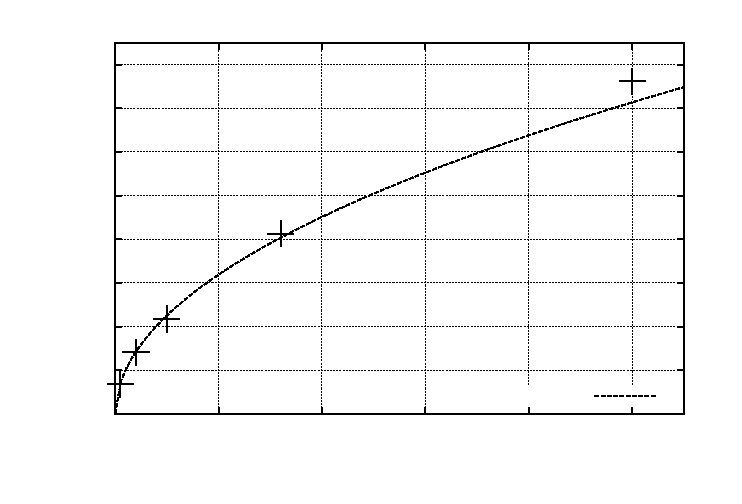
\includegraphics{per}}%
    \gplfronttext
  \end{picture}%
\endgroup

\caption{Doba kmitu v periodickém stavu v závislosti na $C$ pro $R=\SI{20}{\ohm}$}
\label{g:per}
\end{graph}

Hodnoty $L$ v tabulce \ref{t:per} jsme statisticky zpracovali a dostáváme indukčnost cívky $L_1=\SI{0.52(5)}{\henry}$.


\subsection*{Aperiodizační odpor}

Měřili jsme aperiodizační odpor $R_{ap}$ v závislosti na kapacitě $C$.
Chybu aperiodizačního odporu jsme odhadovali tak, abychom pokryli interval, ve kterém jsme nedokázali rozlišit, jestli je průběh proudu periodický či aperiodický.
Uvádíme též hodnotu indukčnosti $L$ vypočtené pro každé měření podle \eqref{e:Laper}.
Odchylku indukčnosti určujeme metodou přenosu chyb jako dvojnásobek relativní chyby aperiodizačního odporu.
Výsledky jsou v tabulce \ref{t:aper} a v grafu \ref{g:aper}.


\begin{tabulka}[htbp]
\centering
\begin{tabular}{c|c|c}
$C$ (\si{\micro\farad}) & $R_{ap}$ (\si{\ohm}) & $L$ (\si{\henry}) \\ \hline
\num{1} & \num{1150(30)} & \num{0.33(2)} \\
\num{3} & \num{665(10)} & \num{0.33(1)} \\
\num{6} & \num{480(10)} & \num{0.35(2)} \\
\num{8} & \num{430(10)} & \num{0.37(2)} \\
\num{10} & \num{370(10)} & \num{0.34(2)} \\
\end{tabular}
\caption{Aperiodizační odpor $R_{ap}$ v závislosti na $C$}
\label{t:aper}
\end{tabulka}

\begin{graph}[htbp] 
\centering
% GNUPLOT: LaTeX picture with Postscript
\begingroup
  \makeatletter
  \providecommand\color[2][]{%
    \GenericError{(gnuplot) \space\space\space\@spaces}{%
      Package color not loaded in conjunction with
      terminal option `colourtext'%
    }{See the gnuplot documentation for explanation.%
    }{Either use 'blacktext' in gnuplot or load the package
      color.sty in LaTeX.}%
    \renewcommand\color[2][]{}%
  }%
  \providecommand\includegraphics[2][]{%
    \GenericError{(gnuplot) \space\space\space\@spaces}{%
      Package graphicx or graphics not loaded%
    }{See the gnuplot documentation for explanation.%
    }{The gnuplot epslatex terminal needs graphicx.sty or graphics.sty.}%
    \renewcommand\includegraphics[2][]{}%
  }%
  \providecommand\rotatebox[2]{#2}%
  \@ifundefined{ifGPcolor}{%
    \newif\ifGPcolor
    \GPcolorfalse
  }{}%
  \@ifundefined{ifGPblacktext}{%
    \newif\ifGPblacktext
    \GPblacktexttrue
  }{}%
  % define a \g@addto@macro without @ in the name:
  \let\gplgaddtomacro\g@addto@macro
  % define empty templates for all commands taking text:
  \gdef\gplbacktext{}%
  \gdef\gplfronttext{}%
  \makeatother
  \ifGPblacktext
    % no textcolor at all
    \def\colorrgb#1{}%
    \def\colorgray#1{}%
  \else
    % gray or color?
    \ifGPcolor
      \def\colorrgb#1{\color[rgb]{#1}}%
      \def\colorgray#1{\color[gray]{#1}}%
      \expandafter\def\csname LTw\endcsname{\color{white}}%
      \expandafter\def\csname LTb\endcsname{\color{black}}%
      \expandafter\def\csname LTa\endcsname{\color{black}}%
      \expandafter\def\csname LT0\endcsname{\color[rgb]{1,0,0}}%
      \expandafter\def\csname LT1\endcsname{\color[rgb]{0,1,0}}%
      \expandafter\def\csname LT2\endcsname{\color[rgb]{0,0,1}}%
      \expandafter\def\csname LT3\endcsname{\color[rgb]{1,0,1}}%
      \expandafter\def\csname LT4\endcsname{\color[rgb]{0,1,1}}%
      \expandafter\def\csname LT5\endcsname{\color[rgb]{1,1,0}}%
      \expandafter\def\csname LT6\endcsname{\color[rgb]{0,0,0}}%
      \expandafter\def\csname LT7\endcsname{\color[rgb]{1,0.3,0}}%
      \expandafter\def\csname LT8\endcsname{\color[rgb]{0.5,0.5,0.5}}%
    \else
      % gray
      \def\colorrgb#1{\color{black}}%
      \def\colorgray#1{\color[gray]{#1}}%
      \expandafter\def\csname LTw\endcsname{\color{white}}%
      \expandafter\def\csname LTb\endcsname{\color{black}}%
      \expandafter\def\csname LTa\endcsname{\color{black}}%
      \expandafter\def\csname LT0\endcsname{\color{black}}%
      \expandafter\def\csname LT1\endcsname{\color{black}}%
      \expandafter\def\csname LT2\endcsname{\color{black}}%
      \expandafter\def\csname LT3\endcsname{\color{black}}%
      \expandafter\def\csname LT4\endcsname{\color{black}}%
      \expandafter\def\csname LT5\endcsname{\color{black}}%
      \expandafter\def\csname LT6\endcsname{\color{black}}%
      \expandafter\def\csname LT7\endcsname{\color{black}}%
      \expandafter\def\csname LT8\endcsname{\color{black}}%
    \fi
  \fi
  \setlength{\unitlength}{0.0500bp}%
  \begin{picture}(6802.00,4534.00)%
    \gplgaddtomacro\gplbacktext{%
      \csname LTb\endcsname%
      \put(1078,704){\makebox(0,0)[r]{\strut{} 0}}%
      \csname LTb\endcsname%
      \put(1078,1213){\makebox(0,0)[r]{\strut{} 200}}%
      \csname LTb\endcsname%
      \put(1078,1723){\makebox(0,0)[r]{\strut{} 400}}%
      \csname LTb\endcsname%
      \put(1078,2232){\makebox(0,0)[r]{\strut{} 600}}%
      \csname LTb\endcsname%
      \put(1078,2741){\makebox(0,0)[r]{\strut{} 800}}%
      \csname LTb\endcsname%
      \put(1078,3250){\makebox(0,0)[r]{\strut{} 1000}}%
      \csname LTb\endcsname%
      \put(1078,3760){\makebox(0,0)[r]{\strut{} 1200}}%
      \csname LTb\endcsname%
      \put(1078,4269){\makebox(0,0)[r]{\strut{} 1400}}%
      \csname LTb\endcsname%
      \put(1210,484){\makebox(0,0){\strut{} 0}}%
      \csname LTb\endcsname%
      \put(2155,484){\makebox(0,0){\strut{} 2}}%
      \csname LTb\endcsname%
      \put(3099,484){\makebox(0,0){\strut{} 4}}%
      \csname LTb\endcsname%
      \put(4044,484){\makebox(0,0){\strut{} 6}}%
      \csname LTb\endcsname%
      \put(4988,484){\makebox(0,0){\strut{} 8}}%
      \csname LTb\endcsname%
      \put(5933,484){\makebox(0,0){\strut{} 10}}%
      \put(176,2486){\rotatebox{-270}{\makebox(0,0){\strut{}$R_{ap}$ (\si{\ohm})}}}%
      \put(3807,154){\makebox(0,0){\strut{}$C$ (\si{\micro\farad})}}%
    }%
    \gplgaddtomacro\gplfronttext{%
      \csname LTb\endcsname%
      \put(5418,877){\makebox(0,0)[r]{\strut{}$R_{ap}=2 \sqrt{L_2/C}$}}%
    }%
    \gplbacktext
    \put(0,0){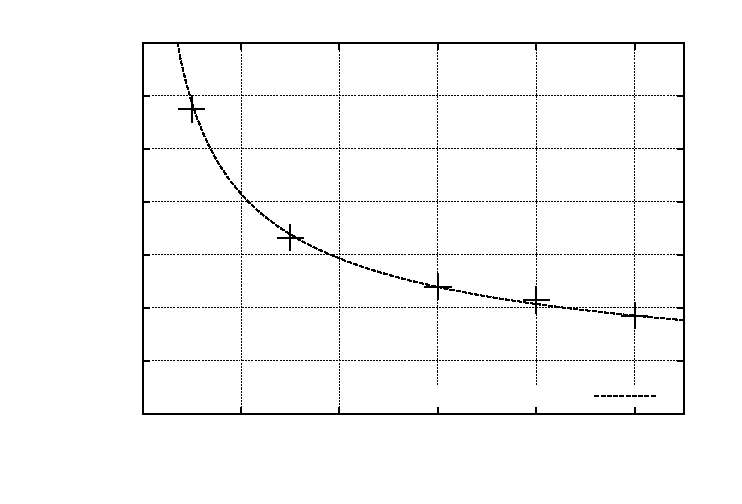
\includegraphics{aper}}%
    \gplfronttext
  \end{picture}%
\endgroup

\caption{Aperiodizační odpor $R_{ap}$ v závislosti na $C$}
\label{g:aper}
\end{graph}

Hodnoty $L$ v tabulce \ref{t:aper} jsme statisticky zpracovali a dostáváme indukčnost cívky $L_2=\SI{0.34(2)}{\henry}$.

\subsection*{RC obvod}

Měřili jsme závislost relaxační doby seriového RC obvodu v závislosti na odporu $R$ a kapacitě $C$.
Změřili jsme několik kapacit pro $R=\SI{1}{\kilo\ohm}$ a pro několik odporů pro $C=\SI{1}{\micro\farad}$.
Programem ISES jsme závislost odporu na čase proložili funkcí ve tvaru $a\cdot\exp(bt)$.
Porovnáním s definičním vztahem relaxační doby získáváme
\begin{equation}
\tau=\frac{-1}{b} \,.
\end{equation}

Výsledky jsou v tabulce \ref{t:RC} a v grafech \ref{g:RCr} a \ref{g:RCc}.
Uvádíme jen hodnoty $\tau$, přímo hodnoty $b$ neuvádíme, případně jsou k nahlédnutí v záznamu z měření.
Kromě změřené hodnoty $\tau$ uvádíme také teoretickou hodnotu $\tau_t$ podle \eqref{e:tau}.

\begin{tabulka}[htbp]
\centering
\begin{tabular}{c|c|c|c}
$C$ (\si{\micro\farad}) & $R$ (\si{\kilo\ohm}) & $\tau$ (\si{\milli\second}) & $\tau_t$ (\si{\milli\second}) \\ \hline
\num{1} & \num{50} & \num{49.2} & \num{50} \\
\num{1} & \num{10} & \num{10.0} & \num{10} \\
\num{1} & \num{4} & \num{3.97} & \num{4} \\
\num{1} & \num{2} & \num{1.96} & \num{2} \\
\num{1} & \num{0.5} & \num{0.514} & \num{0.5} \\
\num{1} & \num{1} & \num{0.962} & \num{1} \\
\num{0.5} & \num{1} & \num{0.523} & \num{0.5} \\
\num{2} & \num{1} & \num{1.92} & \num{2} \\
\num{4} & \num{1} & \num{3.82} & \num{4} \\
\num{6} & \num{1} & \num{5.77} & \num{6} \\
\num{10} & \num{1} & \num{9.60} & \num{10} \\
\end{tabular}
\caption{Závislost relaxační doby $\tau$ na $R$ a $C$}
\label{t:RC}
\end{tabulka}

\begin{graph}[htbp] 
\centering
% GNUPLOT: LaTeX picture with Postscript
\begingroup
  \makeatletter
  \providecommand\color[2][]{%
    \GenericError{(gnuplot) \space\space\space\@spaces}{%
      Package color not loaded in conjunction with
      terminal option `colourtext'%
    }{See the gnuplot documentation for explanation.%
    }{Either use 'blacktext' in gnuplot or load the package
      color.sty in LaTeX.}%
    \renewcommand\color[2][]{}%
  }%
  \providecommand\includegraphics[2][]{%
    \GenericError{(gnuplot) \space\space\space\@spaces}{%
      Package graphicx or graphics not loaded%
    }{See the gnuplot documentation for explanation.%
    }{The gnuplot epslatex terminal needs graphicx.sty or graphics.sty.}%
    \renewcommand\includegraphics[2][]{}%
  }%
  \providecommand\rotatebox[2]{#2}%
  \@ifundefined{ifGPcolor}{%
    \newif\ifGPcolor
    \GPcolorfalse
  }{}%
  \@ifundefined{ifGPblacktext}{%
    \newif\ifGPblacktext
    \GPblacktexttrue
  }{}%
  % define a \g@addto@macro without @ in the name:
  \let\gplgaddtomacro\g@addto@macro
  % define empty templates for all commands taking text:
  \gdef\gplbacktext{}%
  \gdef\gplfronttext{}%
  \makeatother
  \ifGPblacktext
    % no textcolor at all
    \def\colorrgb#1{}%
    \def\colorgray#1{}%
  \else
    % gray or color?
    \ifGPcolor
      \def\colorrgb#1{\color[rgb]{#1}}%
      \def\colorgray#1{\color[gray]{#1}}%
      \expandafter\def\csname LTw\endcsname{\color{white}}%
      \expandafter\def\csname LTb\endcsname{\color{black}}%
      \expandafter\def\csname LTa\endcsname{\color{black}}%
      \expandafter\def\csname LT0\endcsname{\color[rgb]{1,0,0}}%
      \expandafter\def\csname LT1\endcsname{\color[rgb]{0,1,0}}%
      \expandafter\def\csname LT2\endcsname{\color[rgb]{0,0,1}}%
      \expandafter\def\csname LT3\endcsname{\color[rgb]{1,0,1}}%
      \expandafter\def\csname LT4\endcsname{\color[rgb]{0,1,1}}%
      \expandafter\def\csname LT5\endcsname{\color[rgb]{1,1,0}}%
      \expandafter\def\csname LT6\endcsname{\color[rgb]{0,0,0}}%
      \expandafter\def\csname LT7\endcsname{\color[rgb]{1,0.3,0}}%
      \expandafter\def\csname LT8\endcsname{\color[rgb]{0.5,0.5,0.5}}%
    \else
      % gray
      \def\colorrgb#1{\color{black}}%
      \def\colorgray#1{\color[gray]{#1}}%
      \expandafter\def\csname LTw\endcsname{\color{white}}%
      \expandafter\def\csname LTb\endcsname{\color{black}}%
      \expandafter\def\csname LTa\endcsname{\color{black}}%
      \expandafter\def\csname LT0\endcsname{\color{black}}%
      \expandafter\def\csname LT1\endcsname{\color{black}}%
      \expandafter\def\csname LT2\endcsname{\color{black}}%
      \expandafter\def\csname LT3\endcsname{\color{black}}%
      \expandafter\def\csname LT4\endcsname{\color{black}}%
      \expandafter\def\csname LT5\endcsname{\color{black}}%
      \expandafter\def\csname LT6\endcsname{\color{black}}%
      \expandafter\def\csname LT7\endcsname{\color{black}}%
      \expandafter\def\csname LT8\endcsname{\color{black}}%
    \fi
  \fi
  \setlength{\unitlength}{0.0500bp}%
  \begin{picture}(6802.00,4534.00)%
    \gplgaddtomacro\gplbacktext{%
      \csname LTb\endcsname%
      \put(946,704){\makebox(0,0)[r]{\strut{} 0.1}}%
      \csname LTb\endcsname%
      \put(946,1892){\makebox(0,0)[r]{\strut{} 1}}%
      \csname LTb\endcsname%
      \put(946,3081){\makebox(0,0)[r]{\strut{} 10}}%
      \csname LTb\endcsname%
      \put(946,4269){\makebox(0,0)[r]{\strut{} 100}}%
      \csname LTb\endcsname%
      \put(1078,484){\makebox(0,0){\strut{} 0.1}}%
      \csname LTb\endcsname%
      \put(2854,484){\makebox(0,0){\strut{} 1}}%
      \csname LTb\endcsname%
      \put(4629,484){\makebox(0,0){\strut{} 10}}%
      \csname LTb\endcsname%
      \put(6405,484){\makebox(0,0){\strut{} 100}}%
      \put(176,2486){\rotatebox{-270}{\makebox(0,0){\strut{}$\tau$ (\si{\milli\second})}}}%
      \put(3741,154){\makebox(0,0){\strut{}$C$ (\si{\micro\farad})}}%
    }%
    \gplgaddtomacro\gplfronttext{%
      \csname LTb\endcsname%
      \put(5418,877){\makebox(0,0)[r]{\strut{}$\tau=RC$}}%
    }%
    \gplbacktext
    \put(0,0){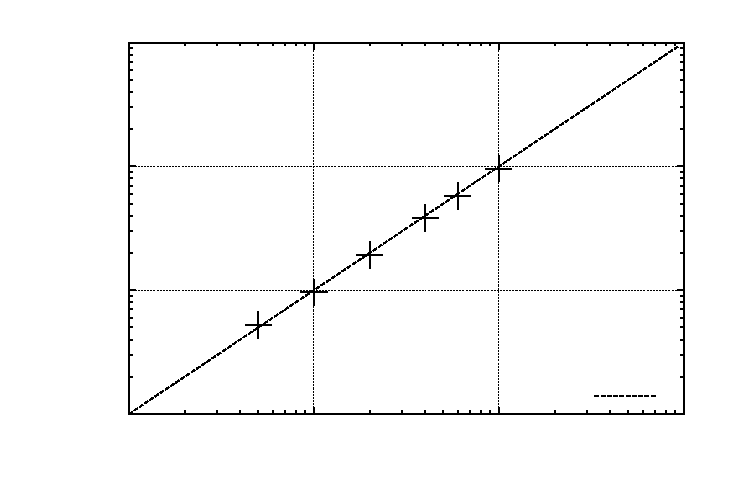
\includegraphics{RCr}}%
    \gplfronttext
  \end{picture}%
\endgroup

\caption{Závislost relaxační doby $\tau$ na $C$ pro $R=\SI{1}{\kilo\ohm}$ (pro přehlednost logaritmické měřítko)}
\label{g:RCr}
\end{graph}

\begin{graph}[htbp] 
\centering
% GNUPLOT: LaTeX picture with Postscript
\begingroup
  \makeatletter
  \providecommand\color[2][]{%
    \GenericError{(gnuplot) \space\space\space\@spaces}{%
      Package color not loaded in conjunction with
      terminal option `colourtext'%
    }{See the gnuplot documentation for explanation.%
    }{Either use 'blacktext' in gnuplot or load the package
      color.sty in LaTeX.}%
    \renewcommand\color[2][]{}%
  }%
  \providecommand\includegraphics[2][]{%
    \GenericError{(gnuplot) \space\space\space\@spaces}{%
      Package graphicx or graphics not loaded%
    }{See the gnuplot documentation for explanation.%
    }{The gnuplot epslatex terminal needs graphicx.sty or graphics.sty.}%
    \renewcommand\includegraphics[2][]{}%
  }%
  \providecommand\rotatebox[2]{#2}%
  \@ifundefined{ifGPcolor}{%
    \newif\ifGPcolor
    \GPcolorfalse
  }{}%
  \@ifundefined{ifGPblacktext}{%
    \newif\ifGPblacktext
    \GPblacktexttrue
  }{}%
  % define a \g@addto@macro without @ in the name:
  \let\gplgaddtomacro\g@addto@macro
  % define empty templates for all commands taking text:
  \gdef\gplbacktext{}%
  \gdef\gplfronttext{}%
  \makeatother
  \ifGPblacktext
    % no textcolor at all
    \def\colorrgb#1{}%
    \def\colorgray#1{}%
  \else
    % gray or color?
    \ifGPcolor
      \def\colorrgb#1{\color[rgb]{#1}}%
      \def\colorgray#1{\color[gray]{#1}}%
      \expandafter\def\csname LTw\endcsname{\color{white}}%
      \expandafter\def\csname LTb\endcsname{\color{black}}%
      \expandafter\def\csname LTa\endcsname{\color{black}}%
      \expandafter\def\csname LT0\endcsname{\color[rgb]{1,0,0}}%
      \expandafter\def\csname LT1\endcsname{\color[rgb]{0,1,0}}%
      \expandafter\def\csname LT2\endcsname{\color[rgb]{0,0,1}}%
      \expandafter\def\csname LT3\endcsname{\color[rgb]{1,0,1}}%
      \expandafter\def\csname LT4\endcsname{\color[rgb]{0,1,1}}%
      \expandafter\def\csname LT5\endcsname{\color[rgb]{1,1,0}}%
      \expandafter\def\csname LT6\endcsname{\color[rgb]{0,0,0}}%
      \expandafter\def\csname LT7\endcsname{\color[rgb]{1,0.3,0}}%
      \expandafter\def\csname LT8\endcsname{\color[rgb]{0.5,0.5,0.5}}%
    \else
      % gray
      \def\colorrgb#1{\color{black}}%
      \def\colorgray#1{\color[gray]{#1}}%
      \expandafter\def\csname LTw\endcsname{\color{white}}%
      \expandafter\def\csname LTb\endcsname{\color{black}}%
      \expandafter\def\csname LTa\endcsname{\color{black}}%
      \expandafter\def\csname LT0\endcsname{\color{black}}%
      \expandafter\def\csname LT1\endcsname{\color{black}}%
      \expandafter\def\csname LT2\endcsname{\color{black}}%
      \expandafter\def\csname LT3\endcsname{\color{black}}%
      \expandafter\def\csname LT4\endcsname{\color{black}}%
      \expandafter\def\csname LT5\endcsname{\color{black}}%
      \expandafter\def\csname LT6\endcsname{\color{black}}%
      \expandafter\def\csname LT7\endcsname{\color{black}}%
      \expandafter\def\csname LT8\endcsname{\color{black}}%
    \fi
  \fi
  \setlength{\unitlength}{0.0500bp}%
  \begin{picture}(6802.00,4534.00)%
    \gplgaddtomacro\gplbacktext{%
      \csname LTb\endcsname%
      \put(946,704){\makebox(0,0)[r]{\strut{} 0.1}}%
      \csname LTb\endcsname%
      \put(946,1892){\makebox(0,0)[r]{\strut{} 1}}%
      \csname LTb\endcsname%
      \put(946,3081){\makebox(0,0)[r]{\strut{} 10}}%
      \csname LTb\endcsname%
      \put(946,4269){\makebox(0,0)[r]{\strut{} 100}}%
      \csname LTb\endcsname%
      \put(1078,484){\makebox(0,0){\strut{} 0.1}}%
      \csname LTb\endcsname%
      \put(2854,484){\makebox(0,0){\strut{} 1}}%
      \csname LTb\endcsname%
      \put(4629,484){\makebox(0,0){\strut{} 10}}%
      \csname LTb\endcsname%
      \put(6405,484){\makebox(0,0){\strut{} 100}}%
      \put(176,2486){\rotatebox{-270}{\makebox(0,0){\strut{}$\tau$ (\si{\milli\second})}}}%
      \put(3741,154){\makebox(0,0){\strut{}$R$ (\si{\kilo\ohm})}}%
    }%
    \gplgaddtomacro\gplfronttext{%
      \csname LTb\endcsname%
      \put(5418,877){\makebox(0,0)[r]{\strut{}$\tau=RC$}}%
    }%
    \gplbacktext
    \put(0,0){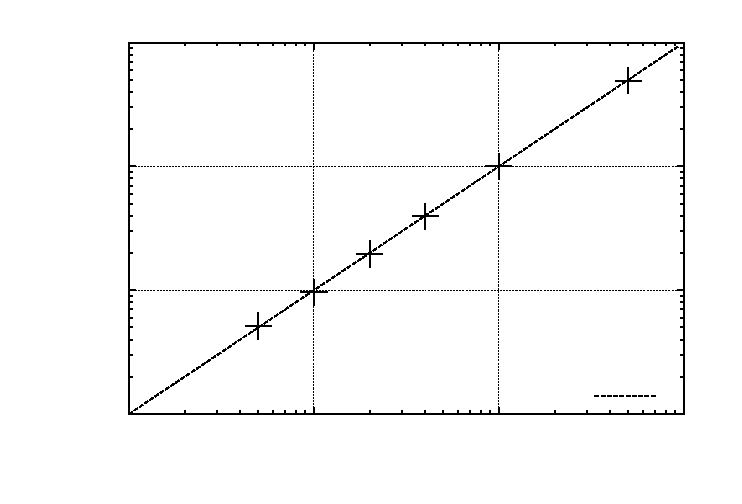
\includegraphics{RCc}}%
    \gplfronttext
  \end{picture}%
\endgroup

\caption{Závislost relaxační doby $\tau$ na $R$ pro $C=\SI{1}{\micro\farad}$ (pro přehlednost logaritmické měřítko)}
\label{g:RCc}
\end{graph}